\chapter{Fermi-Gas freier Elektronen}

\section{Klassisches Drude Modell}

\begin{enumerate}
\item \(e^{-}\) haben keine WW mit dem Gitterpotential
\item \(e^{-}e^{-}\) Wechselwirkung
\item äußere Felder wirken auf die \(e^{-}\)
\item  \(e^{-}\) \(\frac{1}{2}m\langle v^2\rangle =\frac{3}{2}kT\)
\item \(\tau\) Stoßanzahl, Rekombintionszeit \(\frac{1}{\tau}\) \(\frac{dt}{\tau}=\) Wahrscheinlichkeit für Stöße
\end{enumerate}

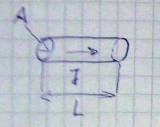
\includegraphics[width=0.75\textwidth]{kap06_17.png}

\(\vec J=\rho j\); \(j=\sigma\vec E\); \(j=\frac{I}{A}\); \(E=\frac{V}{L}\); \(\Rightarrow V=RJ\); \( \frac{\rho L}{A}\)

\[ j = -ne\vec v_D\]

\[\left. \vec v\right|_{t=t_1}=v'_{t=t_0}-\frac{e\vec E t}{m} \]

\begin{align}
\vec v_D &= \langle \vec v \rangle  = \langle v_0\rangle -\frac{eE\tau}{m} \\
&=\frac{eE\tau}{m}
\end{align}


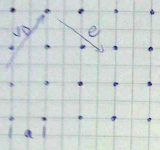
\includegraphics[width=0.75\textwidth]{kap06_18.png}

\(\vec j = \frac{ne^2\tau}{m}\vec E\); \(\sigma = \frac{ne^2\tau}{m}\); \(\tau = \frac{m}{\rho n e^2}\)


\(a\approx 10^{-10}m\); \(\tau = \frac{a}{\sqrt{\langle v\rangle }}\approx \frac{a}{\sqrt{\frac{3k_BT}{m}}}\)
\(\Rightarrow \tau = 10^{-14}s\)

\(\left. a\right|_{300K} = n 10^{23}\); \(\sigma = 10^{5}\frac{1}{\Omega cm}\)

\(\sqrt{\frac{3k_BT}{m}}\approx 10^5\frac{m}{s}\) ; \(l=\frac{\langle v^2\rangle }{\tau}\approx 1 bis 10\cdot 10^{-10}m\)

\(\left. l \right|_{4K}\approx 100\mu m\)

\subsection{Impuls Reelaxation}

\(\vec v = \frac{\vec p}{m} \Rightarrow \vec j = -\frac{ne\vec p}{m}\) Stoßwahrscheinlichkeit: \(\frac{dt}{\tau}\)
keine Stoßwahrscheinlichkeit \(1-\frac{dt}{\tau}\)


\begin{align}
p(t+dt) &= (1-\frac{dt}{\tau})[p(t) + F(t)dt+\mathcal O(dt^2)]\\
&\approx p(t) -\frac{dt}{\tau}p(t) + F(t)dt+\mathcal O(dt^2)
\end{align}

\[\boxed{\frac{dp(t)}{dt}=-\frac{p(t)}{\tau}+F(t)}\]


\underline{Hall-Effekt}
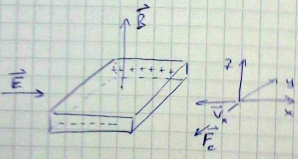
\includegraphics[width=0.75\textwidth]{kap06_19.png}

\[ F = -eE-e\vec v\times \vec B\]

\[E_\gamma = v_xB_z = -\frac{1}{en}j_x B_z = R_H j_xB\]

\[\boxed{R_H=-\frac{1}{en}}\]

Kupfer \(Cq\) - \(R_H=-5,3\cdot 10^{-11}\frac{m^3}{c}\)
Aluminium \(Al\) - \(R_H=+9,9\cdot 10^{-11}\frac{m^3}{c}\)



\begin{align}
\frac{dp}{dt} &= -eE - \frac{e}{m}\vec p \times \vec B - \frac{\vec p}{\tau} = 0\\
0&=-eE_x - \frac{e}{m}p_yB - \frac{p_x}{\tau}\\
0&=-eE_y - \frac{e}{m}p_xB - \frac{p_y}{\tau}
\end{align}

\[ \Rightarrow \sigma E_x = \omega_c \tau j_y + j_x\]
\[ \Rightarrow \sigma E_y = -\omega_c \tau j_y + j_y\]

Zyklotronfrequenz
\[ \omega_c = \frac{e}{m}B \]

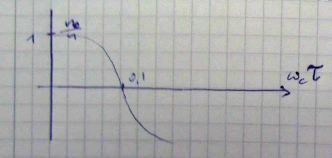
\includegraphics[width=0.75\textwidth]{kap06_20.png}

Laut Drude sollte \(\omega_C\tau \propto B\) sein, ist es aber nicht (warum, nicht kapito)

\subsection{Wechselstromleitfähigkeit}

\(\frac{dp}{dt} = -\frac{\vec p}{\tau} - e\vec E\); \(E(t) = Re\{E(\omega)e^{-i\omega t}\}\)

Versuch der Lösung

\[ p(t) = - Re\{p(\omega)e^{-i\omega t}\} \]
\( -i\omega \vec p(\omega) = -\frac{\vec p(\omega)}{\tau}-e\vec E\); \(\vec j = -\frac{ne}{m}\vec p\)
\(\Rightarrow j(t) =  Re\{j(\omega)e^{-i\omega t}\}\)

\[ j(\omega) = -\frac{ne}{m} p(\omega) = \frac{ne^2}{m}\frac{\vec E(\omega)}{\frac{1}{\tau}-i\omega}\equiv\sigma(\omega)\vec E(\omega) \]

\[\boxed{\sigma(\omega) = \frac{\sigma_0}{1-i\omega\tau}}\]

Magnetfeld \(H(\omega) \approx 0\); \(\frac{v}{c}<< 1\); \(v_D\approx 10^{-3}\frac{m}{s}\)

Maxwell-Gleichungen \(\lambda = \frac{2\pi c}{\omega}>> e \)
Ampersche Gesetz: \(\vec \nabla \times \vec H = j + \epsilon_0\frac{\partial E}{\partial t}\)

\begin{align}
\vec \nabla \times \vec \nabla \times \vec E = -\nabla^2 E &= i\omega \mu_0\sigma \vec E - i\omega \epsilon_0\vec E\\
&=w^2 \epsilon_0\mu_0\epsilon(\omega) \vec E
\end{align}

\[\epsilon (\omega) = 1+ \frac{i\sigma(\omega)}{\epsilon_0 \omega}\]


\begin{enumerate}
\item hohee Frequenzen \(\sigma(\omega) = \omega_0\frac{1+i\omega\tau}{1+\omega^2\tau^2}\approx\sigma_0\frac{i}{\omega\tau}\); \(\Rightarrow \epsilon(\omega) = 1-\frac{\sigma_0}{\epsilon_0\tau\omega^2}=\frac{\omega^2_0}{\omega^2}\)

Die Plasmafrequenz, ist gerade die Frequenz wo die \(e^-\)  dem Feld noch folgen können. 
\[ \omega_p = \frac{ne^2\tau}{m\epsilon_0 \tau}=\frac{ne^2}{m\epsilon_0}\]
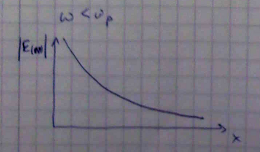
\includegraphics[width=0.75\textwidth]{kap06_21.png}

\item kleine Frequenzen \(\omega\tau << 1\)

\[\sigma (\omega) = \sigma_0 \frac{1+i\omega\tau}{1+\omega^2\tau} =  \sigma_0(1+i\omega\tau)\]

\[ \epsilon(\omega) = 1+\sigma(mega)\frac{1}{\epsilon_0\omega} = 1 + \sigma_0(\underbrace{\frac{i}{\epsilon_0\omega}}_{\epsilon_2}-\underbrace{\frac{\tau}{\epsilon_0}}_{\epsilon_1})\]

\[ \epsilon(\omega) = = i\epsilon_2\]

\[ k = \frac{\omega}{c}\sqrt{\epsilon(\omega)} =  \frac{\omega}{c}\sqrt{\frac{\sigma_0}{\epsilon_0 \omega}}\frac{1+i}{\sqrt 2} = \frac{1}{s}(1+i)\]

\[s = c\sqrt{\frac{2\epsilon_0}{\sigma_0\omega}}\]

\(s\) ist der Skin oder Leitschichtdicke (Dimension Länge) oder der Skin-Effekt. Der Strom fließt nun noch an der Oberfläche des Leiters. 

\end{enumerate}


1853 Widermann-Franz. Die Wärmeleitfähigkeit und die Leitfähigkeit ist zur Temperatur proportional:

\[ \frac{\kappa}{\sigma} = LT\]

\(L\)-Loreznzahl zwischen \(2,2-2,8\cdot 10^{-3}\frac{\omega\Omega}{K^2}\)

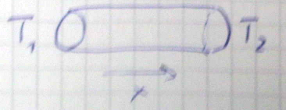
\includegraphics[width=0.75\textwidth]{kap06_22.png}

\(j^T = \kappa \nabla T\)

\begin{align}
j^T_x &= \langle \frac{1}{2}v_x [u_x(x-v\tau)i-u_c(x+v\tau]\rangle \\
&= n\langle v_x^2\rangle \tau \frac{du_e}{dT}(-\frac{dT}{dx}
\end{align}

\(c_v = n\frac{du}{dT}\); \(\rangle v^2\rangle  = \langle v_x^2\rangle = \langle v^2_x\rangle =\langle v_z^2\rangle \)

\[ j^T = \underbrace{\frac{1}{3}v^2\tau c_v}_{\kappa = \frac{1}{3}v^2\tau c_v=\frac{1}{3}lvc_v} \]

\[ LT =  \frac{\kappa}{\sigma} = \frac{c_v}{ne^2} \frac{mv^2}{3} \]
\(\Rightarrow c_v = \frac{3}{2} nk_B\)

\[ L =\frac{\kappa}{\sigma}\frac{3}{2} nk_B \frac{k^2_B}{K^2} T = 1,1\cdot 10^{-3}\frac{\omega\Omega}{K^2}\frac{mv^2}{2} = \frac{3}{2}k_B T\]

tatsächlich: \(c^2_v\) Fatkro 100 kleiner, \(v^2\) ist ein Faktor 100 größer



\section{Sommerfeld-Theorie der Metalle}

Klassische, Ideales Gas Maxwell-Bolzmann Veirteilung

\[ f_{MG} = (v) = n\left(\frac{m}{2\pi kT}\right)^{3/2}e^{-\frac{mv^2}{k_B T}} \]

Pauliprinzip:

Fermi Dirac Verteilung

\[ f_{FD} = f(v) = \left(\frac{m}{2\pi \hbar}\right)^3 \frac{2}{e^{\frac{mv^2/2-\mu}{k_BT}}+1} \]

\(n=\int_V f(v) dV\); \(k_BT_0 = \nu\)

Zustandsdichte des freien Elektronen Gases:

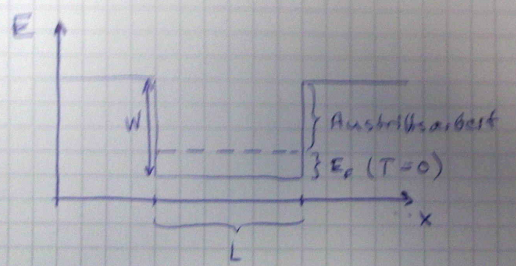
\includegraphics[width=0.75\textwidth]{kap06_23.png}

N Elektronen
SchrGl: \(-\frac{\hbar}{2m} \nabla \psi(\vec r) = E \psi(\vec r)\); \(\psi(\vec r) = \frac{1}{\sqrt{V}} e^{-\vec k\vec r}\); \(1=\int_V|\psi(\vec r)|^2dV\); \(E=\frac{\hbar^2k^2}{2m}\);

Peridizitätsbedingung:  \(\psi(x,y,z) = \psi(x+L,y,z)\)

\(k_i=\frac{2\pi}{L}m_i\) \(i=x,y,z\); \(m=1,2,3\)

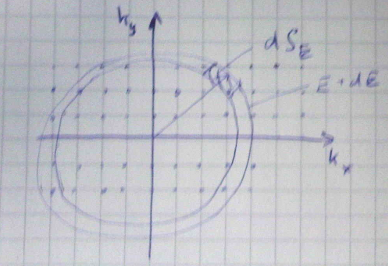
\includegraphics[width=0.75\textwidth]{kap06_24.png}

\[\mathcal D(E) dE = \frac{V}{(2\pi)^3}\int^{E+dE}_E d^3 k = \frac{V}{(2\pi)^3} \frac{1}{\hbar} \int_{E=const.} \frac{dS_E}{v_g}\]

\(\rho_x = \frac{V}{(2\pi)^3}\)

Gruppengeschwindigkeit: \(v_g = \frac{\partial E}{\partial(\hbar k} = \frac{\hbar k}{m}\)

Randbemerkung: \(\frac{1}{v_g}\int dS_E = \frac{1}{v_g}-4\pi k^2\)

\[\mathcal D_\uparrow(E) = \frac{V}{(2\pi)^3}\frac{1}{\hbar} \frac{m}{\hbar k}4\pi k^2 = \frac{(2m)^{3/2}}{4\pi^2\hbar^2} V\sqrt{E}\]

Volumen normierte und mit 2 \(e^-\) besetzte Zustandsdichte:

\[ \mathcal D(E) = \frac{1}{V} (\mathcal D_\uparrow + \mathcal D_\downarrow) = \frac{(2m)^{3/2}}{2\pi^2\hbar^2}\sqrt{E}\]

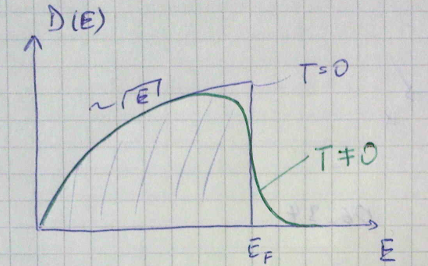
\includegraphics[width=0.75\textwidth]{kap06_25.png}

\(\rho^\propto_k=\left(\frac{L}{2\pi}\right)^\propto\)

\(D^{2D}=\frac{m}{\pi \hbar^2}\); \(D^{1D}(E) = \frac{1}{\pi\hbar} \sqrt{\frac{2}{E}}\)

\[f(E,T=0) = \begin{cases}
  1: & E<\mu \\
  \frac{1}{2}: & E=\mu \\
  0: & E>\mu 
\end{cases}
\]

\(\mu = \left(\frac{\partial F}{\partial N}\right)_{T,V}=E_F(T=0)\)

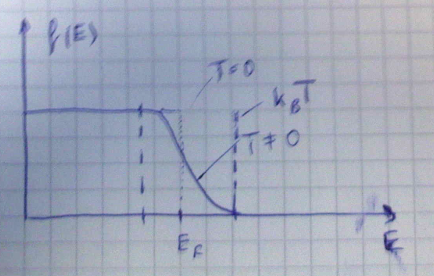
\includegraphics[width=0.75\textwidth]{kap06_26.png}

\[n=\frac{N}{V}=\int_0^\infty \mathcal D(E) f(E,0)dE = \int_0^{E_F}\]

\[E_F = \frac{\hbar^2}{2m}(3\pi^2n)^{2/3}\]

Fermi-Energie: \(E_F = \frac{\hbar^2}{2m}(3\pi^2 n)^{2/3}\) mit Elektronendichte \(n=\frac{N}{V}\)
Fermi-Wellenvektor \(k_F=(3\pi^2n)^{1/3}\)
Fermi Impuls: \(p_F = \hbar k_F\)
Fermi-Geschwindigkeit \(v_F = \frac{\hbar}{m}(3\pi^2 n)^{1/3}\)
Fermi Temperatur \(T_F = \frac{E_F}{k_B}\)


\begin{tabular}{cccccc}
&\(n/10^{6}m^{-3}\)&\(k_f/A^{-1}\)&\(v_F10^{6}\frac{m}{s}\)&\(E_F/eV\)&\(FT/K_F\)\\
Al&18,1&1,8&2,0&11,7&135000\\
Cu&8,5&1,4&1,6&7,0&82000\\
Ag&5,9&1,2&1,4&5,5&64000
\end{tabular}


\[\boxed{\mu(T)\approx E_F [1-\frac{\pi^2}{12}\left(\frac{T}{T_F}\right)^2]}\]


TODO Einleitende Abbildungen möglich am anfang von Sommerfeldtheorie einfügen


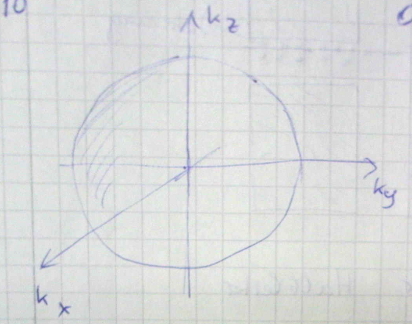
\includegraphics[width=0.75\textwidth]{kap06_27.png}


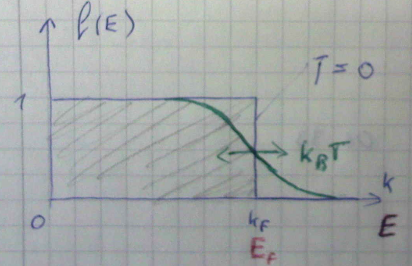
\includegraphics[width=0.75\textwidth]{kap06_28.png}
Kurze Einleitung was die Quantennatur der Theorie ist (Pauliprinzip, Besetzung in der Fermikugel, nur an der Fermikante befindliche elektronen sind relevant für verschiedene Effekte)

\subsection{Spezifische Wärme}

\(c_V = \frac{\partial }{\partial T}U(T)\) mit \(U\) als innere Energie

\begin{align}
c_V &= \frac{\partial }{\partial T}U(T)\\
&= \frac{\partial }{\partial T}\int_0^\infty ED(E)f(E,T)dE\\
&=\frac{\partial }{\partial T}\frac{1}{2\pi^2}\left(\frac{2m}{\hbar}\right)^{3/2}\int_0^\infty\frac{E^{3/2}dE}{e^{\frac{E-\mu}{k_BT}}-1}
\end{align}

\begin{align}
D(E)&=\frac{(2m)^{3/2}\sqrt{E}}{2\pi^2\hbar^3}\\
&=\frac{3}{2}n\sqrt{E}\left[\frac{\hbar^2}{2m}(3\pi^2 n)^{2/3}\right]^{-3/2}\\
&= \frac{3}{2}\frac{n}{E_F}\left(\frac{E}{E_F}\right)^{1/2}
\end{align}


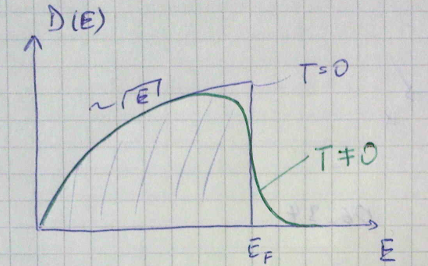
\includegraphics[width=0.75\textwidth]{kap06_25.png}

'grobe'-Rechnung:

\begin{align}
U(0) &= \int_0^{E_F}ED(E)dE\\
&= \frac{3}{2}\frac{n}{E_F^{3/2}}\frac{2}{5}E^{5/2}\\
&=\frac{3n}{5}E_F\\
&=\frac{3n}{5}k_BT
\end{align}

Temperaturabhängige Anteil der innerer Inergie:

\[\delta U(T) = U(T)-U(0) \approx nk_BT\frac{T}{T_F} = nk_B \frac{T^2}{T_F}\]

\(\frac{T^2}{T_F}\) der Bruchteil der Elektronen der die thermische Energie \(k_BT\) pro Elektron aufnehmen kann

\(c_V \approx \frac{\partial}{\partial T}[\delta U(T)] = \frac{2nk_BT}{T_F}\) ist um Faktor \(\frac{T}{T_F}\) kleiner als mit einem klass. Gas.

exaktere Näherungslösung:  \(U(T) \approx U(0) +\frac{\pi^2}{6}D(E_F)(k_BT)^2\); \(c_V=\gamma T\); mit Sommerfeldkonstanten \(\gamma = \frac{\pi^23nk_B}{3T_F2}\)

Die gesamte spezifische Wärme:

\[c_V^{\text{ges}} = c_V^{el}+c_V^{ph} = \gamma T + \begin{cases}
 \beta T^3,  & T<<\theta_D\\
 3R=const,  & T>\theta_D
\end{cases}\]


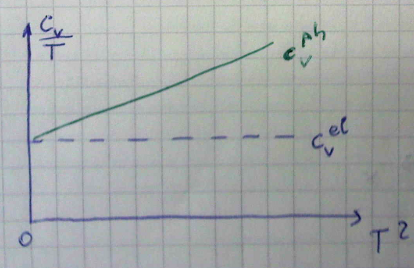
\includegraphics[width=0.75\textwidth]{kap06_30.png}

Offene Fragen nach Sommerfeld-Modell:

\begin{enumerate}
\item Warum collidieren \(e^-\)-nen nicht mit Ionen?
\item Warum teilen/unterscheiden wir zwischen Metalle, Halbleiter, Isolatoren?
\item Warum wechselwirken  \(e^-\)-nen nicht mit einander?
\end{enumerate}

Die ersten zwei Fragen sind von Bloch-Theorie beantwortet. Die dritte Frage - Fermi-Flüssigkeiten (komplizierte QM-Theorie)



